\chapter{Experimental Setting}
\label{chapter:Experimental Setting}

This chapter provides information about the experimental setting for the evaluation of the proposed method Batch Deep COACH (BD-COACH). Experiments are done both in simulation with a simulated teacher and in a real setup with a human teacher.


\section{Meta-World benchmark}
\label{section:Meta-World Benchmark}
To evaluate BD-COACH and compare its performance to the base method D-COACH, we use three simulated environments from the open-source benchmark Meta-World \cite{metaworld}. Meta-World 
provides 50 standardized manipulation tasks that use a simulated Sawyer robot arm. Even if this benchmark was specifically designed for multi-task and meta-reinforcement learning, it is possible to simply access single goal environments as we do for this thesis. All Meta-World tasks are implemented in the MuJoCo physics engine \cite{mujoco} and it is interfaced with OpenAI Gym \cite{openai} making it easy to use. 
For each task, Meta-World includes an oracle policy that commands the best action for the environment at a given time step. This action is equal to 
$[\delta x, \delta y, \delta z, \textrm{gripper effort}]$
where a value of 1 for the gripper effort keeps the fingers of the end effector open whereas a value of -1 closes them.



In order to properly evaluate the method under controlled conditions, a high performance policy teacher provided by the Meta-World benchmark was used. The simulated teacher generates feedback computing $h = \operatorname{sign}(a_\text{teacher} - a_\text{agent})$, whereas the decision on whether to provide feedback at each time step is given by the probability $P_h = \alpha \cdot \operatorname{exp}(-\tau \cdot \operatorname{time step})$, where $\{\alpha \in \mathbb{R}\, | 0 \leq \alpha \leq 1 \}$; $\{\tau \in \mathbb{R} \, | 0 \leq \tau\}$. Furthermore, this binary feedback $h$ is only provided if the difference between the action of the policy and the action of the teacher is smaller than a threshold $\theta$.

The Meta-World benchmark defines a success metric as the evaluation criterion for their tasks. This metric, ${\left\lVert \text{object}-\text{goal} \right\rVert}_2 < \epsilon$, is based on the euclidean distance between the object position and the goal position where $\epsilon$ is a small distance threshold that varies from task to task.




\subsection{Task plate-slide-v2}
\label{subsection:metaworld-hockey-task}

The sequence of the plate-slide-v2 task can be seen in Figure \ref{fig:sequence-plate-slide}; the gripper of the end effector has to approach the puck, press it vertically and then slide the puck to the goal. If the puck goes inside the goal in less than 500 time steps, the episode is considered successful and a fail otherwise. The task starts with the gripper and the object always initiated at the same position whereas the goal is initiated randomly within an area of  $0.01m^2$. During all the episode the gripper remains closed as the policy teacher commands a gripper effort of $-1$.


The success metric that Meta-World defines for this task is ${\left\lVert \text{object}-\text{goal} \right\rVert}_2 < 0.07$.

 \begin{figure}[H]
  \centering
  \hspace*{\fill}%
  \subfloat[1 - Approach to puck]{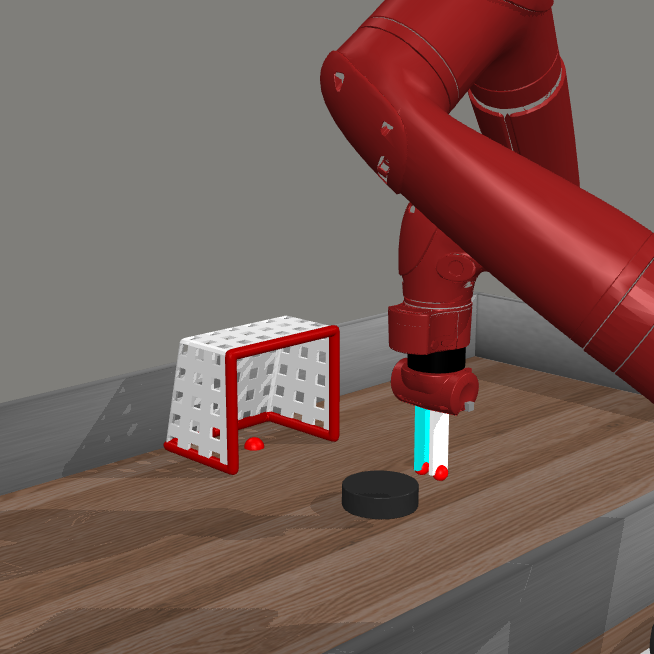
\includegraphics[width=0.25\textwidth]{figures/hockeypos0_v2.png}\label{fig:hockey_pos_0}}
   \hfill
  \subfloat[2 - Press puck vertically]{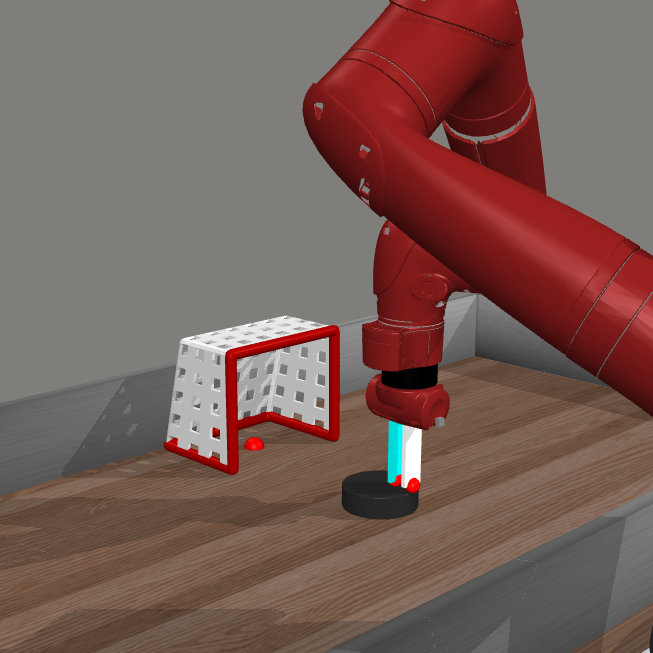
\includegraphics[width=0.25\textwidth]{figures/hockeypos1_v2.png}\label{fig:hockey_pos_1}}
   \hfill
  \subfloat[3 - Slide puck to goal]{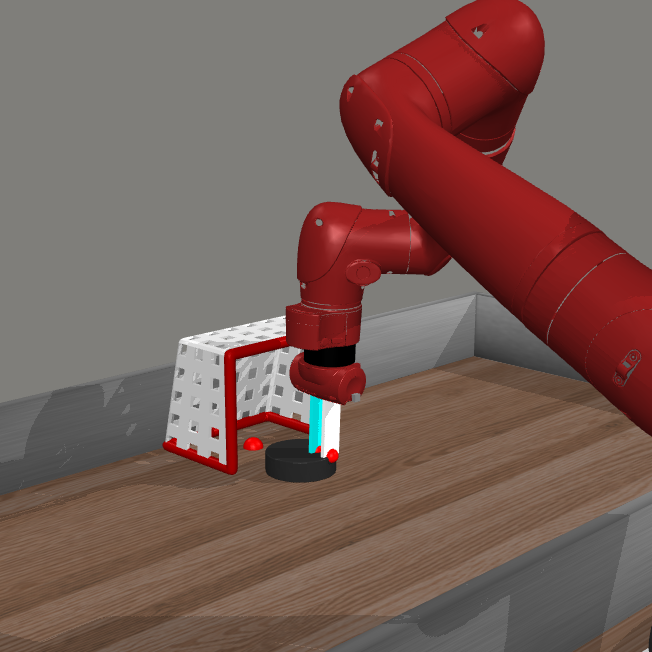
\includegraphics[width=0.25\textwidth]{figures/hockeypos2_v2.png}\label{fig:hockey_pos_2}}
  \hspace*{\fill}%
  \caption{Sequence of the plate-slide-v2 task in Meta-World}.
  \label{fig:sequence-plate-slide}
\end{figure}


\subsection{Task drawer-open-v2}
\label{subsection:metaworld-open-drawer-task}


The second simulated Meta-World task is called drawer-open-v2, see Figure \ref{fig:sequence-drawer}. For an episode to be considered a success, the end effector has to approach the handle of the drawer which is always initiated closed, hook to it and pull to open it in less that 500 time steps.
For this task the gripper remains open during all the episode as the gripper effort commanded by the simulated teacher is always 1. The gripper is initiated always at the same position and the drawer can appear at a random position within a length of $0.2m$. The success metric for this task is ${\left\lVert \text{object}-\text{goal} \right\rVert}_2 < 0.03$.
 




 \begin{figure}[H]
  \centering
  \hspace*{\fill}%
  \subfloat[1 - Approach to handle]{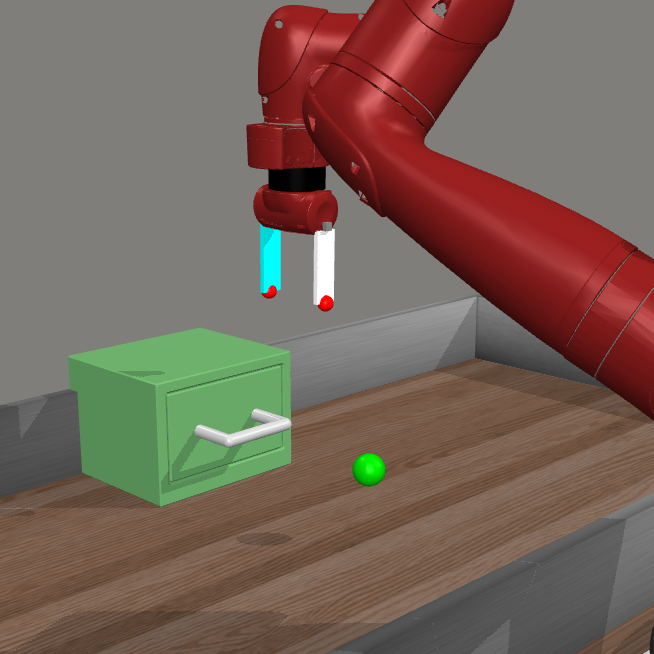
\includegraphics[width=0.25\textwidth]{figures/drawerpos0_v2.png}\label{fig:drawer_pos_0}}
   \hfill
  \subfloat[2 - Hook handle]{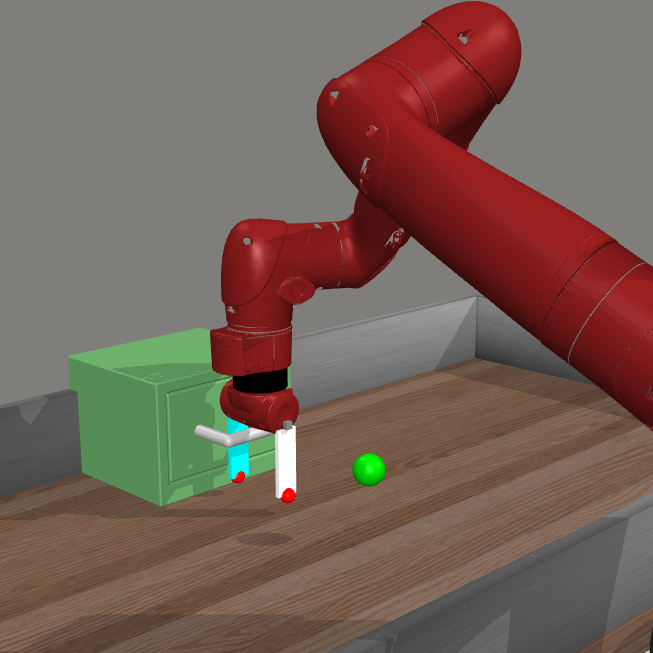
\includegraphics[width=0.25\textwidth]{figures/drawerpos1_v2.png}\label{fig:drawer_pos_1}}
   \hfill
  \subfloat[3 - Open drawer]{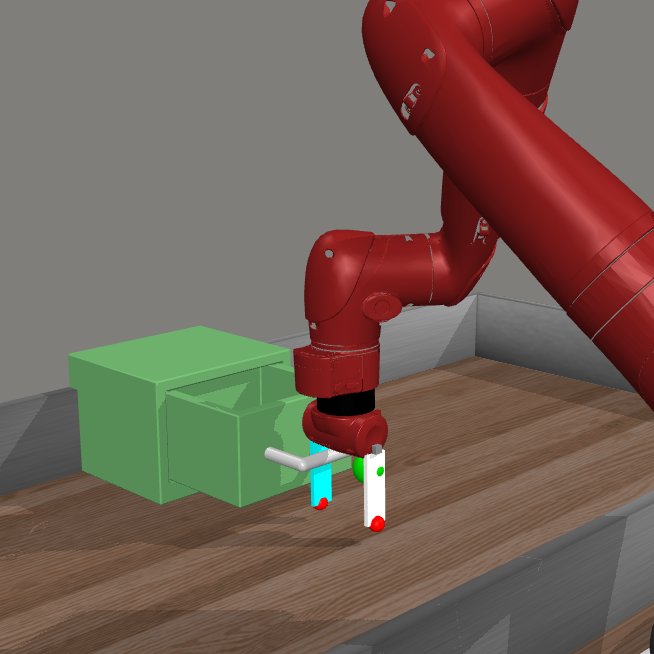
\includegraphics[width=0.25\textwidth]{figures/drawerpos2_v2.png}
  \label{fig:drawer_pos_2}}
  \hspace*{\fill}%
  \caption{Sequence of the drawer-open-v2 task in Meta-World}.
  \label{fig:sequence-drawer}
\end{figure}


\subsection{Task button-press-topdown-v2}
\label{subsection:metaworld-button-press-topdown-v2}

The final simulated Meta-World task is called button-press-topdown-v2, see Figure \ref{fig:sequence-button}. For an episode to be considered a success, the end effector has to reach the button which is placed perpendicular to the surface of the table, and press it vertically in less that 500 time steps.
For this task the gripper remains closed during all the episode as the gripper effort commanded by the simulated teacher is always -1. The gripper is initiated always at the same position whereas the button is initiated randomly within an area of  $0.02m^2$.The success metric for this task is ${\left\lVert \text{object}-\text{goal} \right\rVert}_2 < 0.02$.

 \begin{figure}[H]
  \centering
  \hspace*{\fill}%
  \subfloat[1 - Approach to button]{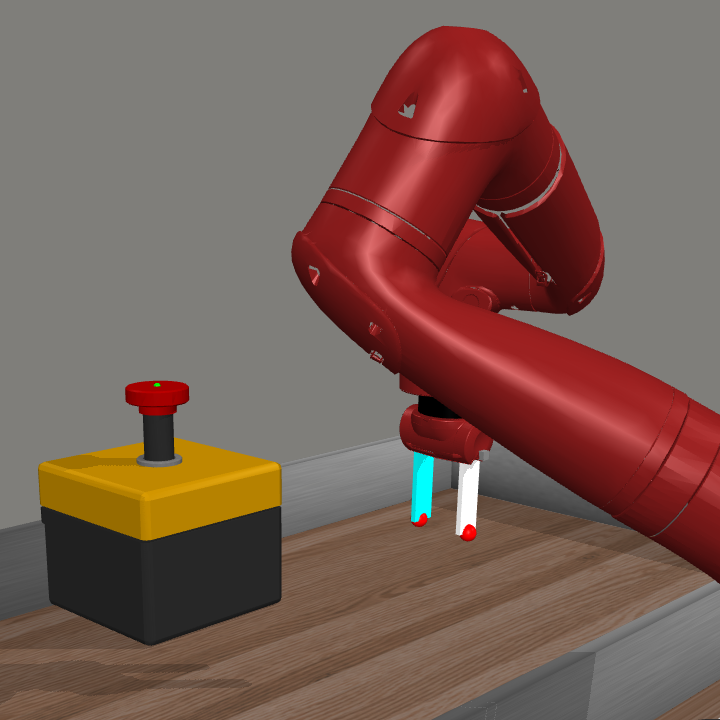
\includegraphics[width=0.25\textwidth]{figures/button_1.png}\label{fig:button_pos_0}}
   \hfill
  \subfloat[2 - Reach button]{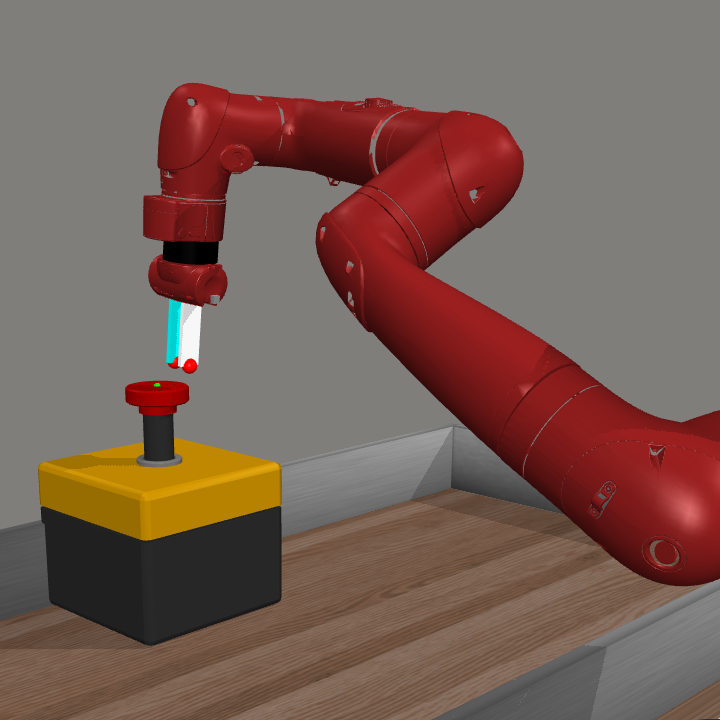
\includegraphics[width=0.25\textwidth]{figures/button_2.png}\label{fig:button_pos_1}}
   \hfill
  \subfloat[3 - Press button vertically]{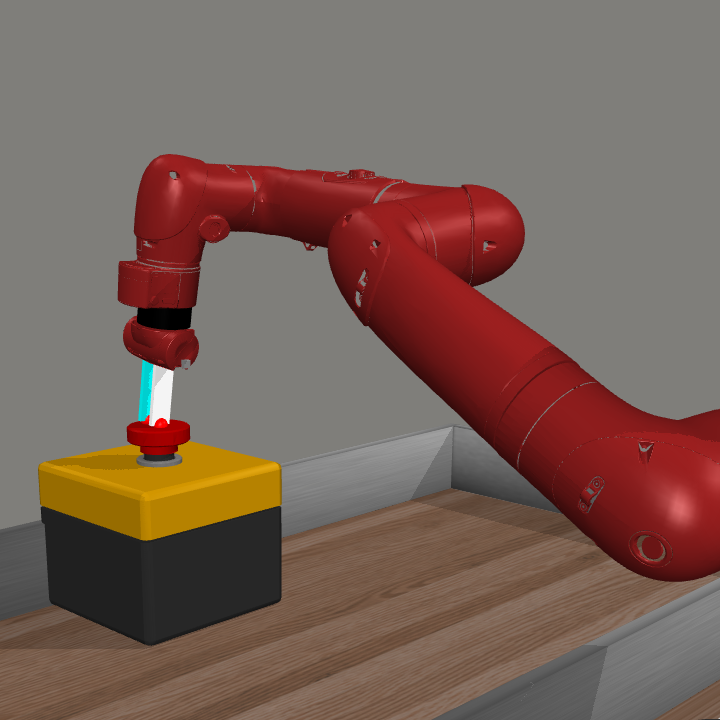
\includegraphics[width=0.25\textwidth]{figures/button_3.png}
  \label{fig:button_pos_2}}
  \hspace*{\fill}%
  \caption{Sequence of the button-press-topdown-v2 task in Meta-World}.
  \label{fig:sequence-button}
\end{figure}


\begin{table}[H]
\centering
\renewcommand{\arraystretch}{1.4}
\begin{tabular}{llS[table-format=2.2]SSS[table-format=2.2]S[table-format=2.2]}
\toprule
\textbf{Parameter }& \textbf{Value}\\[-.4em]
\midrule
Policy hidden sizes  &   (256, 128)\\
Policy activation of hidden layers  &   (tanh, tanh)\\
Policy learning rate  &  0.001\\
Human model hidden sizes &   (512, 512)\\
Human model activation of hidden layers  &   (tanh, tanh)\\
Human model learning rate  &   0.001\\
Buffer sampling rate&   10\\
Buffer sampling size &   20\\
Max time steps per episode &   500\\
\bottomrule
\end{tabular}
\caption{Hyperparameters used for the experiments}
\label{tab:hyperparameters}
\end{table}



\section{Experiments with KUKA robot arm}
\label{section:Experiments with KUKA robot arm}

In order to validate the new proposed method BD-COACH on a real robotic setup, we devised two tasks involving a KUKA LBR iiwa 7 robot arm pushing a box placed on top of a table; These 2 tasks will be explained later in more detail.

Several reflecting markers were attached to the box so its pose could be tracked by an OptiTrack motion capture system. The pose captured by the 8 cameras of the available OptiTrack system, consists on the position and orientation of the center point on the box created by the reflecting markers. 

The human that supervises the learning process conveys the corrections with a joystick. In order to make the task easier to teach, the human provides corrections just in the 2 axis parallel to the surface of the table while the vertical position of the end effector is kept constant and close to the surface of the table. Prior to perform the real experiments, everything was checked in a simulated Gazebo environment.

A ROS network connects all the required elements for the experiment, these being: The feedback corrections from the joystick, the pose of the box from the optitrack and the position of the end effector of the KUKA. Specifically, for retrieving the position and sending the commands to the robot arm, the iiwa ROS stack \cite{iiwa} is used. For the control of the arm, we chose the control from the stack called \textit{CustomControllers}. It allows the control of the end effector in the Cartesian space and its command is formed by 6 values where the first 3 values are the orientation of the end effector ant the last 3 values, its position. For our purposes, we fix the orientation and the position in the vertical axis. The requested command in the remaining 2 positions is the current position of the end effector plus a delta which is the output of the network. Therefore, the policy outputs a 2 dimensional actions representing the relative changes to the positions in the axes parallel to the table.

Regarding the state that enters to the policy, it is a 7 dimensional array whose components are: 1- The relative position between the end effector and the box in the x axis (axis parallel to the length of table).
2 - The relative position between the end effector and the box in the z axis (axis parallel to the width of the table).
3 - Velocity of the end effector in the x axis.
4 - Velocity of the end effector in the z axis.
5 - Position of the box in the x axis.
6 - Position of the box in the z axis.
7 - Orientation of the box (The pitch angle perpendicular to the surface of the table).

Finally, a simple metric of success is implemented. This metric has a value of 1 if the box ends within a small radius from the target position and 0 otherwise.

\subsection{Task push-box}
\label{subsection:Push box in a straight line}

For the first task called push-box, the KUKA arm has to push a box placed on one side of the table to a goal position indicated with a green cross. This task that may seem trivial at first glance is known as the \textit{planar manipulation problem} \cite{constant_velocity} and it really highlights the importance of reactive robots. It is challenging because it involves an unstable system. If the goal is to push an object in a straight line with a pushing interaction, with a non-reactive robot, this task is simply impossible to achieved as the box will naturally fall outside the desired straight trajectory. 

 Figure \ref{fig:planar-motion-problem} shows this problem. A constant velocity is commanded to the end effector but because the robot does not react to the misalignments, the box keeps deviating from the desired straight trajectory.


 \begin{figure}[H]
  \centering
  \hspace*{\fill}%
  \subfloat{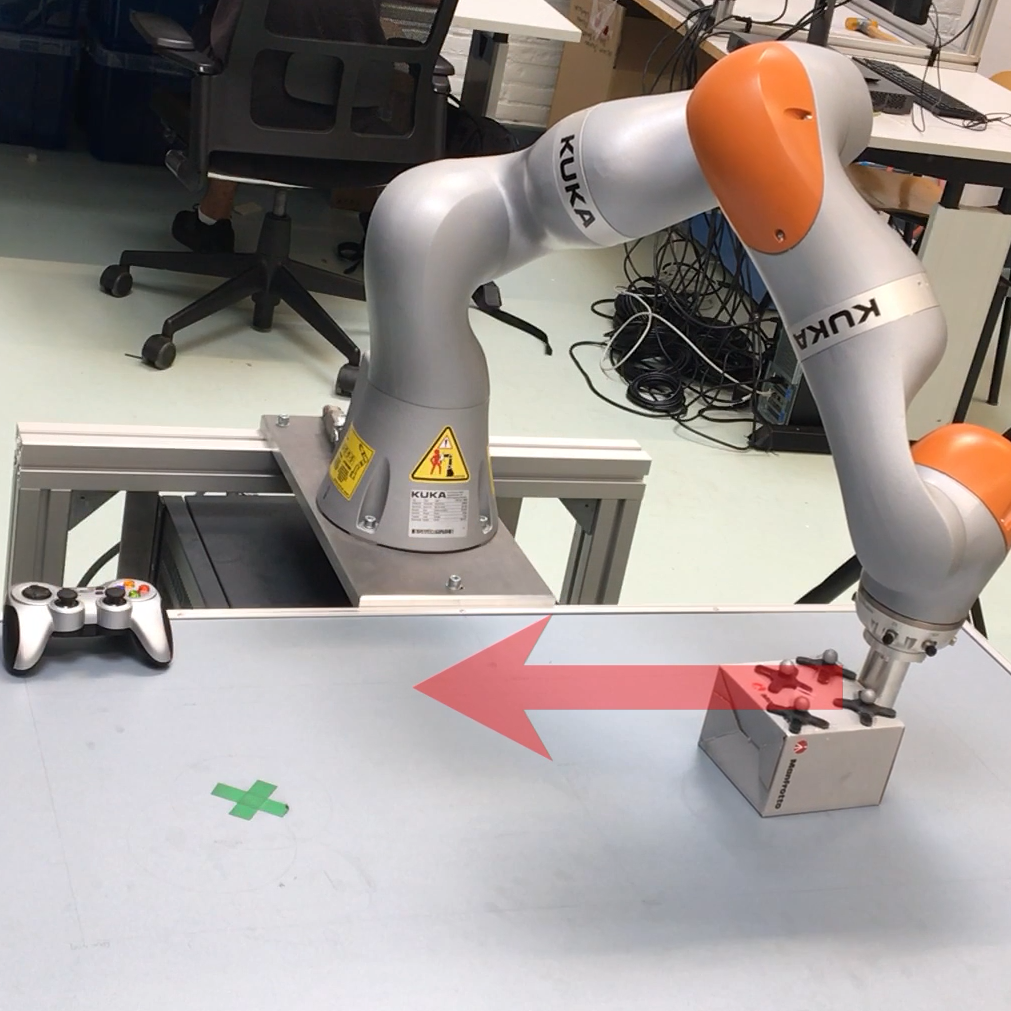
\includegraphics[width=0.25\textwidth]{figures/const_vel0.png}\label{fig:drawer_pos_0}}
   \hfill
  \subfloat{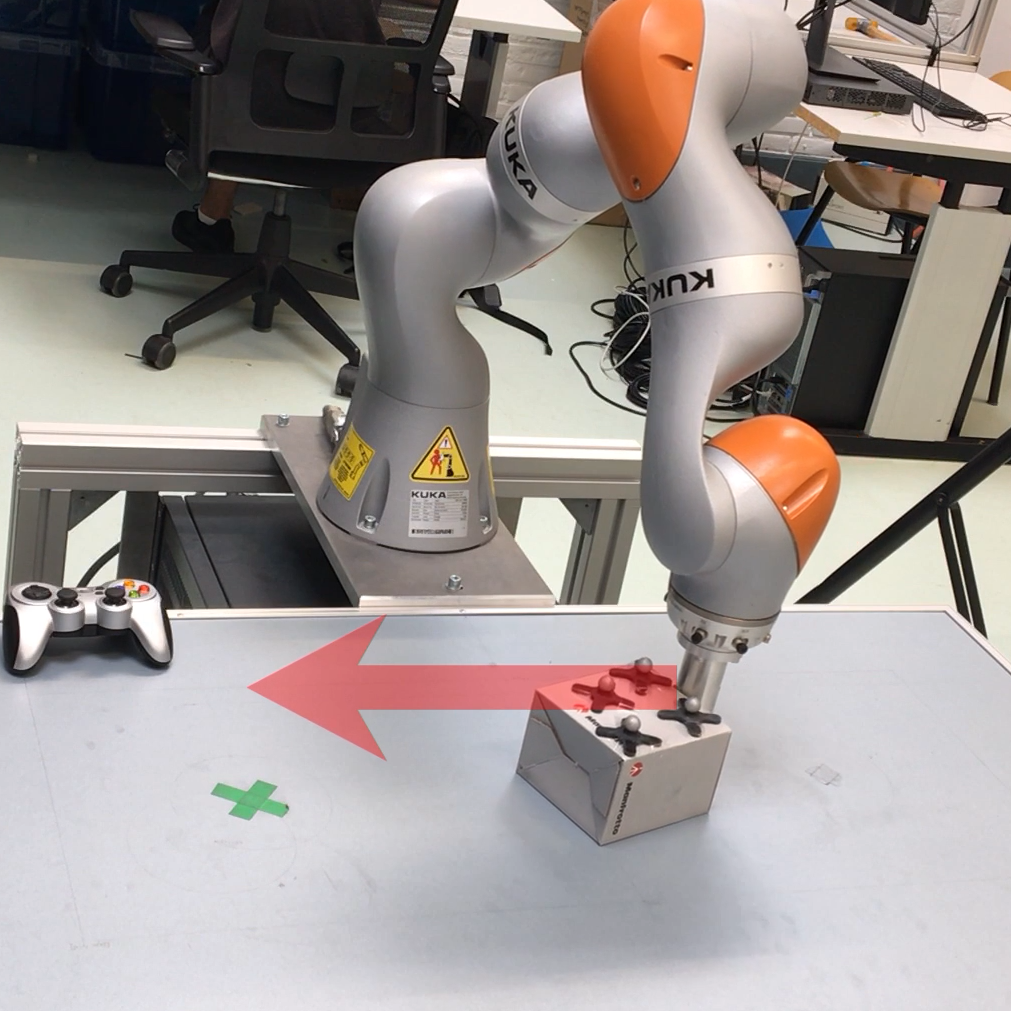
\includegraphics[width=0.25\textwidth]{figures/const_vel1.png}\label{fig:drawer_pos_1}}
   \hfill
  \subfloat{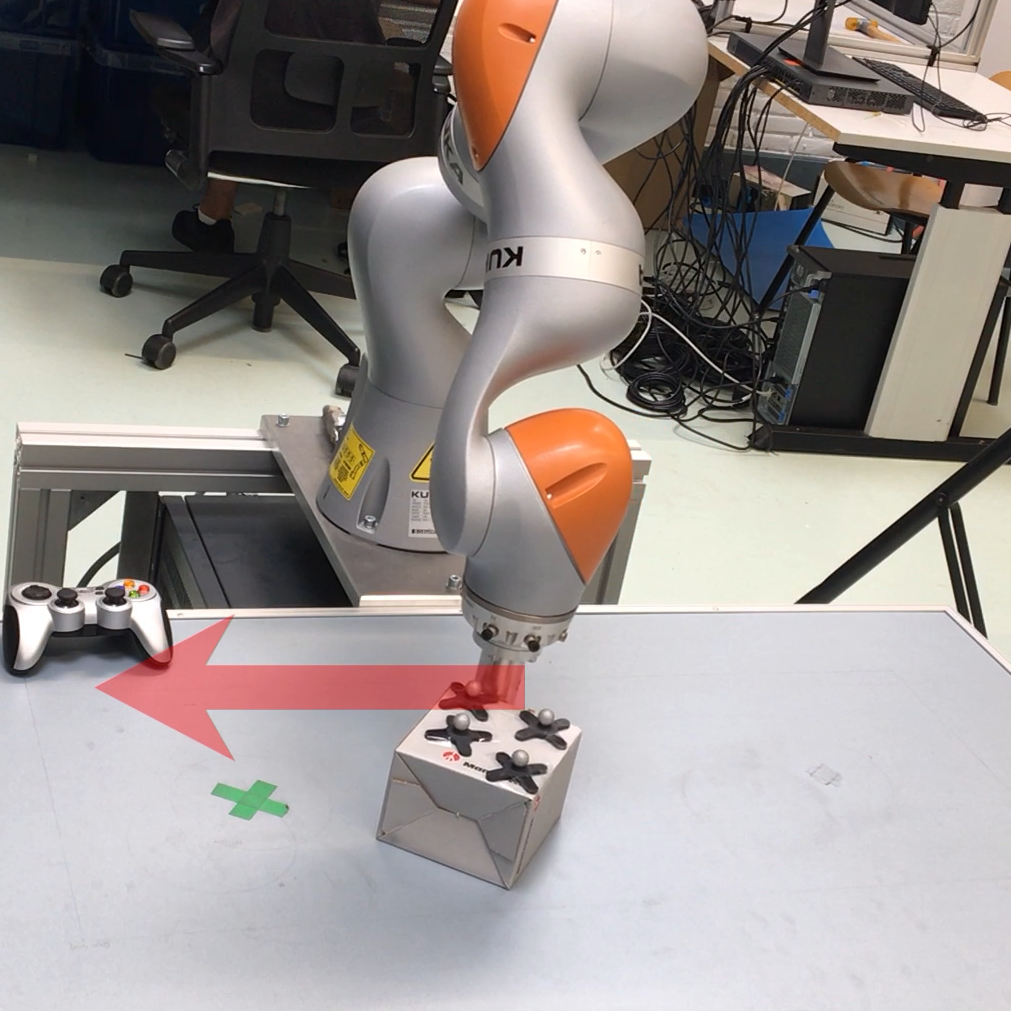
\includegraphics[width=0.25\textwidth]{figures/const_vel2.png}\label{fig:drawer_pos_2}}
   \hspace*{\fill}%
  \caption{By applying a constant velocity, the box gets easily misaligned.}
  \label{fig:planar-motion-problem}
\end{figure}

Figure \ref{fig:sequence-push-box} shows a sequence of the task once the agent has been trained using BD-COACH. The box is initialized at random positions and disturbances are manually introduced. The agent is able to succesfully reach the goal by learning a continuous back and forth motion that makes possible to quickly correct the misalignments of the box when it starts changing its orientation.

 \begin{figure}[H]
  \centering
  \subfloat[1 - Start position]{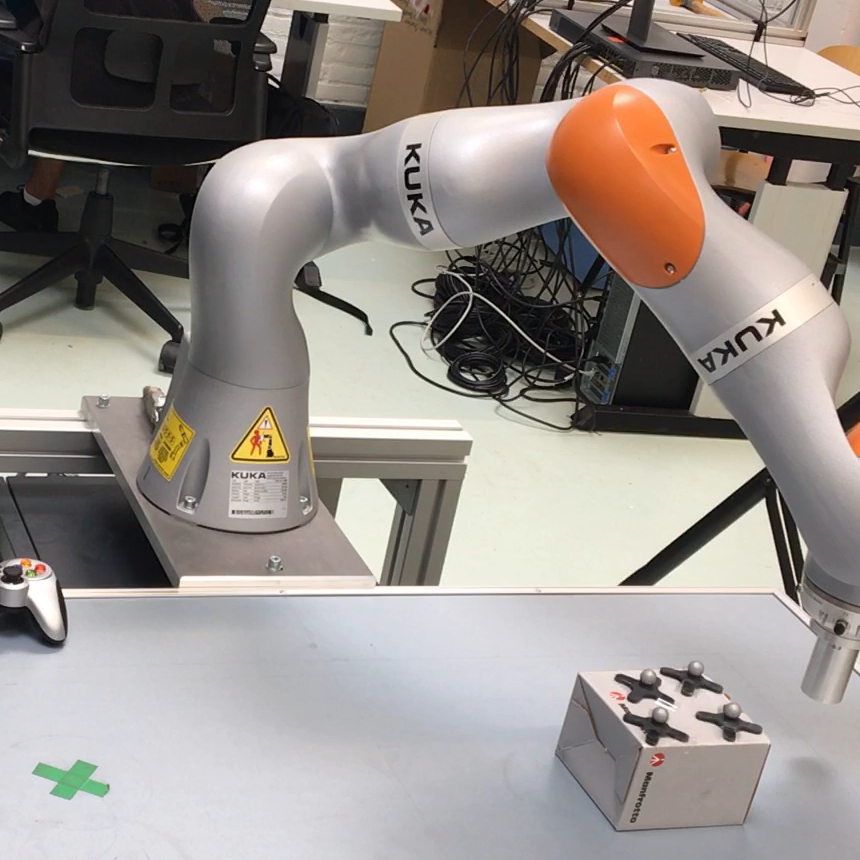
\includegraphics[width=0.19\textwidth]{figures/push0.png}\label{fig:push_pos_0}}
   \hfill
  \subfloat[2 - Approach to box]{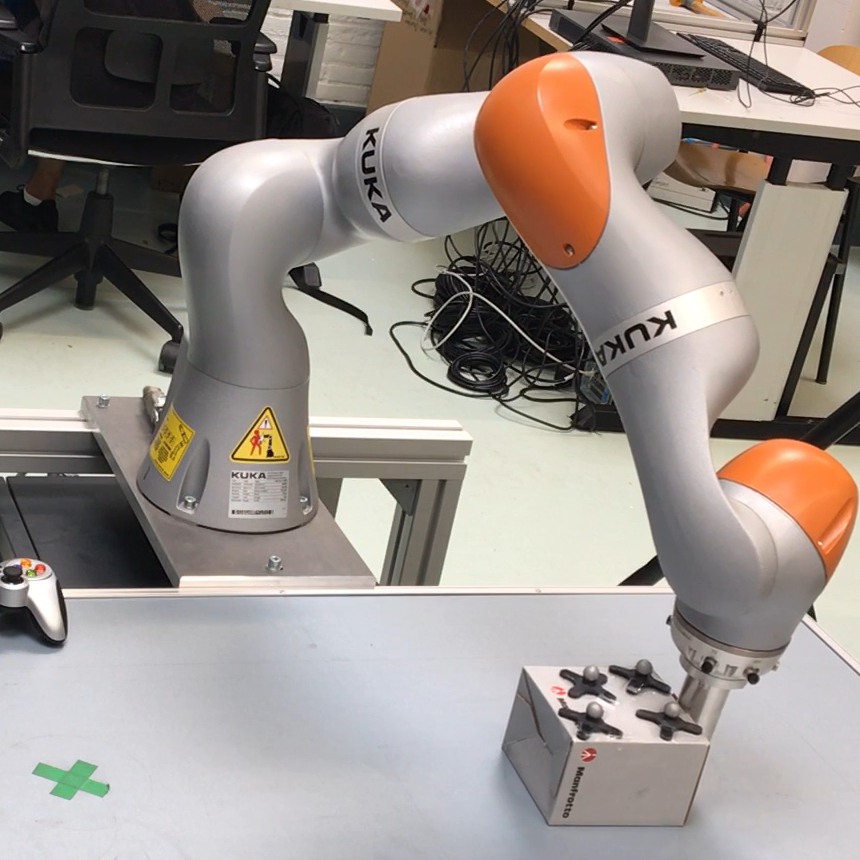
\includegraphics[width=0.19\textwidth]{figures/push1.png}\label{fig:push_pos_1}}
   \hfill
  \subfloat[3 - Introduce disturbance]{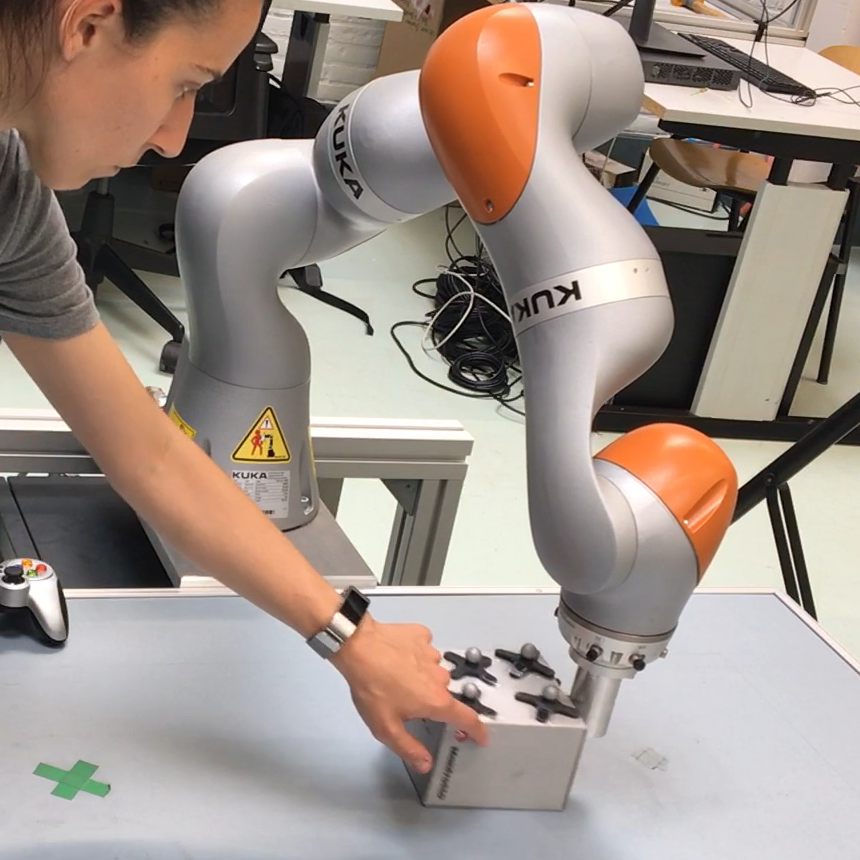
\includegraphics[width=0.19\textwidth]{figures/push2.png}\label{fig:push_pos_2}}
   \hfill
  \subfloat[4 - Correct disturbance]{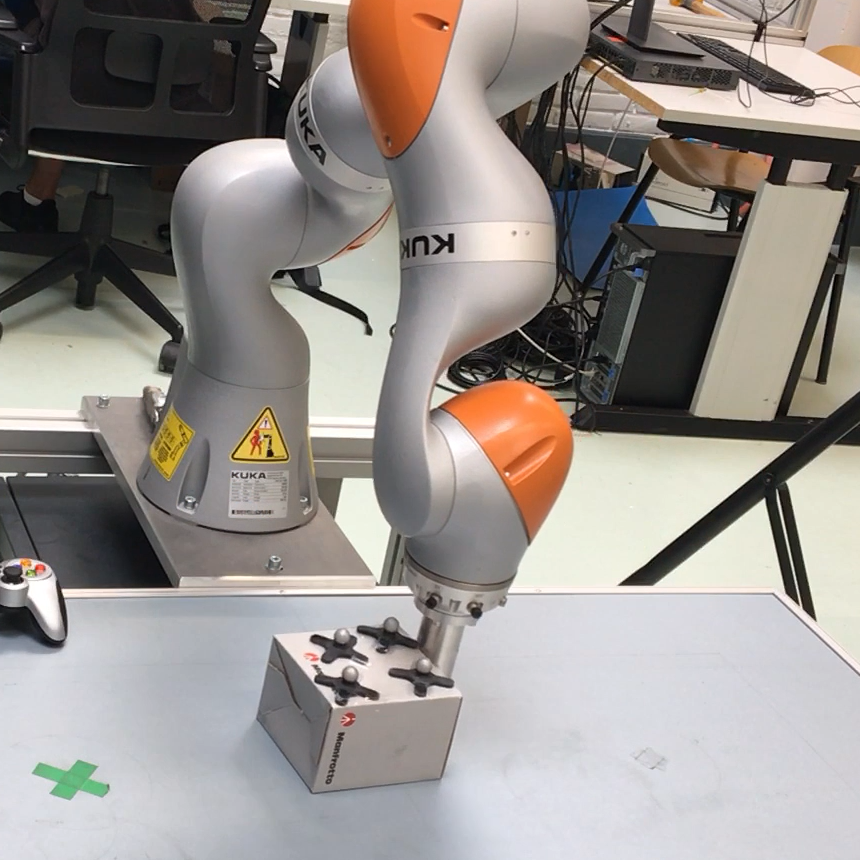
\includegraphics[width=0.19\textwidth]{figures/push3.png}\label{fig:push_pos_2}}
   \hfill
  \subfloat[5 - End position]{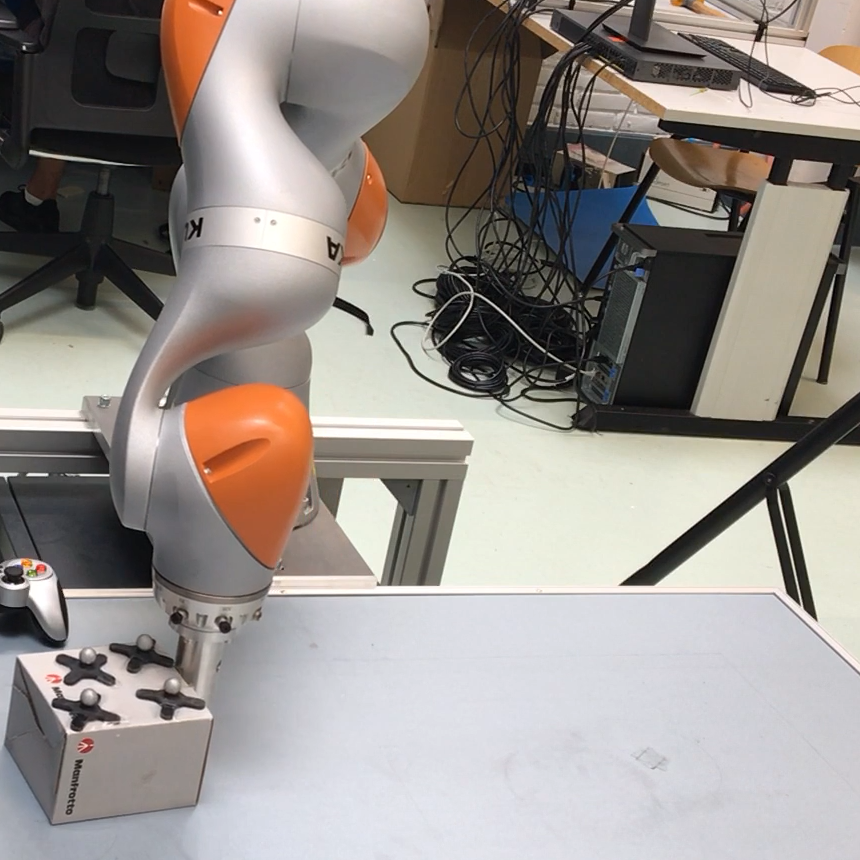
\includegraphics[width=0.19\textwidth]{figures/push5.png}\label{fig:push_pos_2}}
  \caption{Sequence of the task push-box}.
  \label{fig:sequence-push-box}
\end{figure}







\subsection{Task park-box}
\label{subsection:Park a box}

The second task also involves pushing a box but this time the sequence of movements is more complex. To achieve the goal, the robot has to push is both axes parallel to the surface of the table. Once it has pushed it and center it until it faces the 2 brown boxes (third frame of Figure \ref{fig:sequence-park-box}), the end effector moves around the corner of the pink box and starts pushing from the other side until the box is fit between the 2 walls. Figure \ref{fig:sequence-park-box} shows the sequence of movements for this task.


 \begin{figure}[H]
  \centering
  \subfloat[1 - Start position]{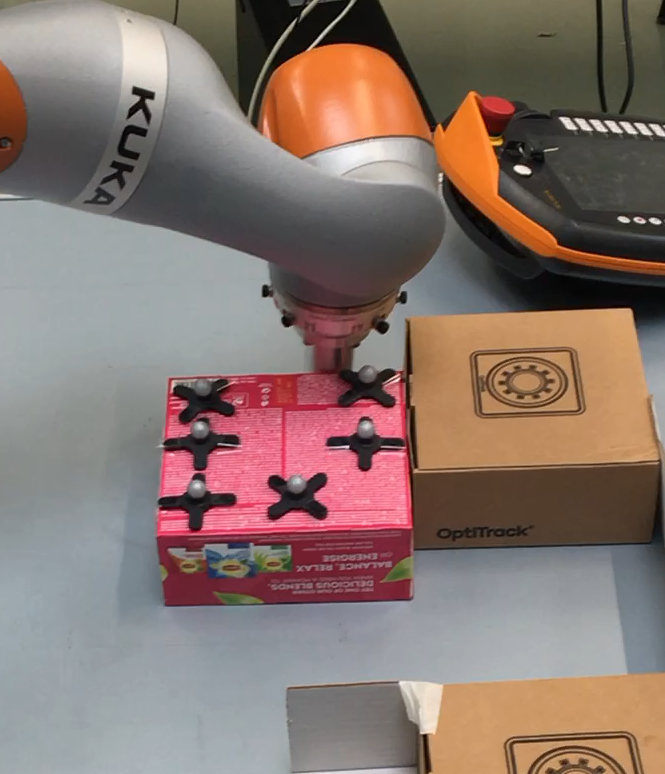
\includegraphics[width=0.16\textwidth]{figures/park0_v2.png}\label{fig:drawer_pos_0}}
   \hfill
  \subfloat[2 - Push box]{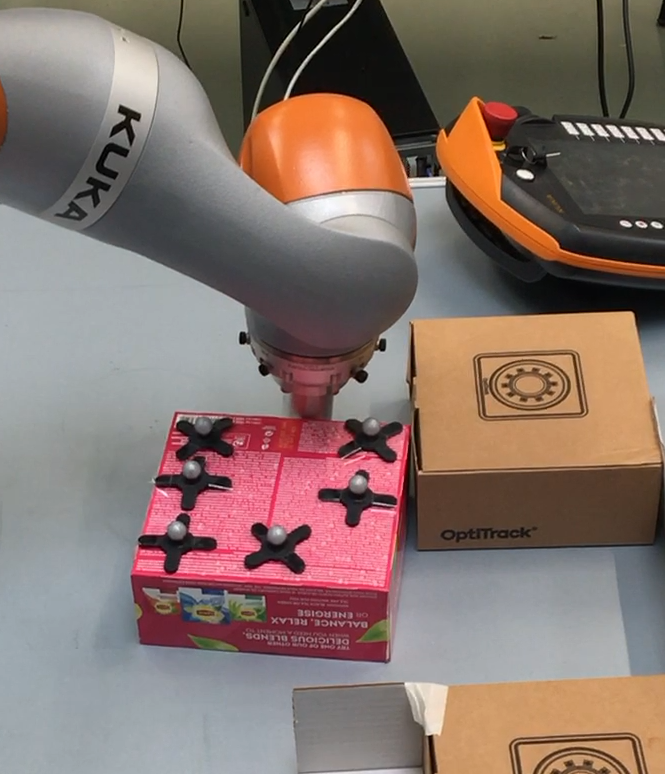
\includegraphics[width=0.16\textwidth]{figures/park1_v2.png}\label{fig:drawer_pos_1}}
   \hfill
  \subfloat[3 - Center box]{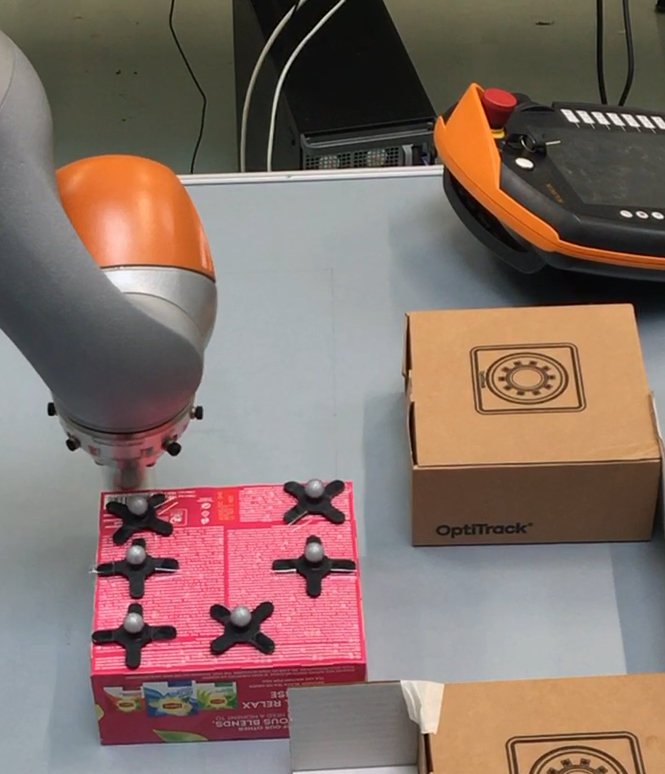
\includegraphics[width=0.16\textwidth]{figures/park3_v2.png}\label{fig:drawer_pos_2}}
   \hfill
  \subfloat[4 - Move around corner]{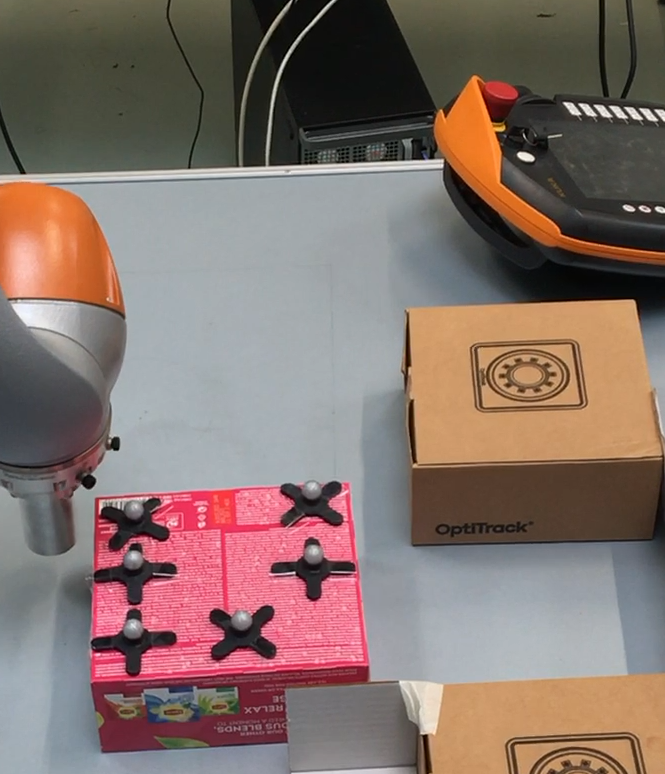
\includegraphics[width=0.16\textwidth]{figures/park4_v2.png}\label{fig:drawer_pos_2}}
   \hfill
  \subfloat[5- Push box between walls]{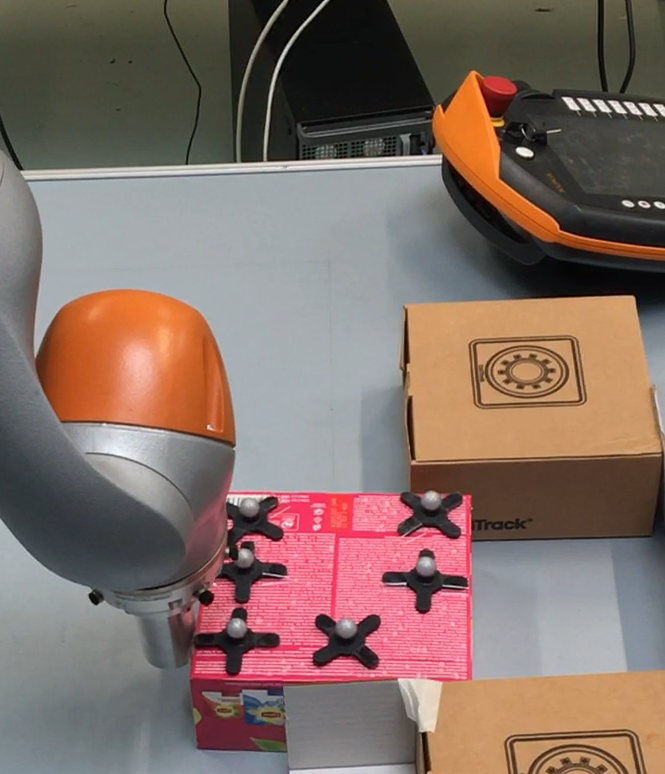
\includegraphics[width=0.16\textwidth]{figures/park5_v2.png}\label{fig:drawer_pos_2}}
   \hfill
  \subfloat[6 - End position]{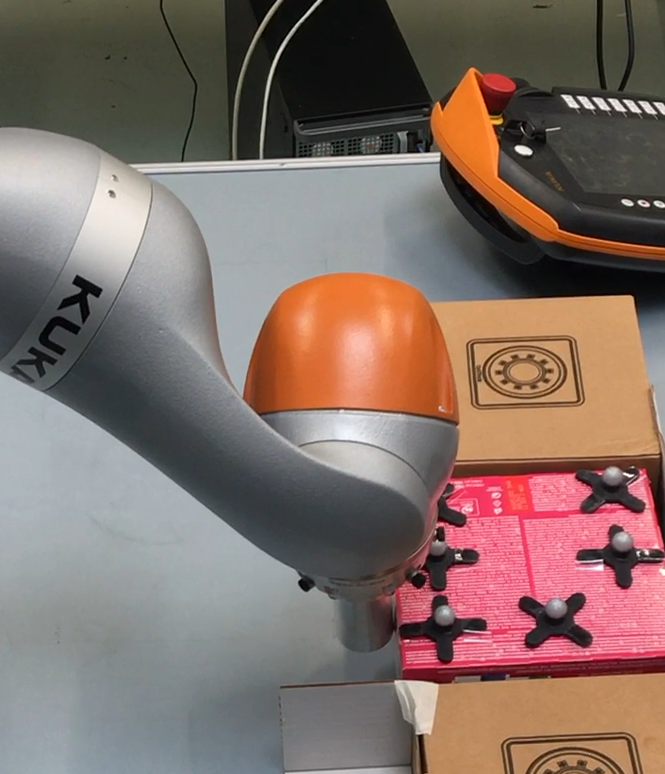
\includegraphics[width=0.16\textwidth]{figures/park6_v2.png}\label{fig:drawer_pos_2}}
  \caption{Sequence of the task park-box}.
  \label{fig:sequence-park-box}
\end{figure}

